%%%%%%%%%%%%%%%%
% Info on beamer: 
% 1) http://en.wikibooks.org/wiki/LaTeX/Presentations
% 2) Mertz2005
% 3) Rivero2012
%%%%%%%%%%%%%%%

%%%%%%%%%%%%%%%%%%%%%%%%%%%%%%%%
% this Latex template should be stored in: ~/Library/TeXShop/Templates
%%%%%%%%%%%%%%%%%%%%%%%%%%%%%%%%

\documentclass[xcolor=pdftex, dvipsnames, table]{beamer}
% have a look at page 38 onwards of the documentation for the `xcolor` package in order to see predefined color names

% a couple of built-in themes
%\usetheme{Warsaw}
%\usetheme{Berkeley}
\usecolortheme{dolphin}

% suppress the navigation bar:
\beamertemplatenavigationsymbolsempty	

% packages:
\usepackage{booktabs} % for tables
\usepackage{natbib} % for citations
\usepackage{hyperref} % for hyperlinks
\usepackage{amssymb} % for mathematical symbols
%\usepackage{beamerthemesplit}
% others to try: beamerthemebars, beamerthemelined, beamerthemetree, beamerthemetreebars

% \usepackage{beamerthemesplit} // Activate for custom appearance

% Note, paths need to end with a forward slash "/"
\graphicspath{ 
{/Users/Claudius/Documents/PhD/THESIS/kks32/LaTeX/Presentations/Group_meeting/figures/} 
{/Users/Claudius/Documents/PhD/THESIS/kks32/LaTeX/Data_analysis/reference-mapping/figure/}
{/Users/Claudius/Documents/PhD/PhDupgradeReport/}
{/Users/Claudius/Documents/PhD/Marie-Curie-ITN/Groningen09/ProjectPresentation/}
{/Users/Claudius/Documents/PhD/sRAD/sRAD_Analysis/}
}

\title{Incomplete digestion}
\subtitle{troubleshooting RAD library prep \vskip80pt}
%\author{  Claudius Kerth\inst{1} }
\institute{
\raggedright
{\large{Claudius Kerth}}\\
%	\inst{1}
%	Animal and Plant Science Department, \\
%	Sheffield University\\
%	Arthur Willis Environment Centre\\
	\vskip15pt
	\hskip4pt
	\textit{c.kerth@shef.ac.uk}
}
\date{ \raggedright \small{24 Feb 2015}}


%%%%%%%%%%%%%
\begin{document}
%%%%%%%%%%%%%

%%%%%%%%%%%%%%%%%%%%%%%%
% Create Title page
%%%%%%%%%%%%%%%%%%%%%%%%
% Local background must be enclosed by curly braces for grouping.
{
\usebackgroundtemplate{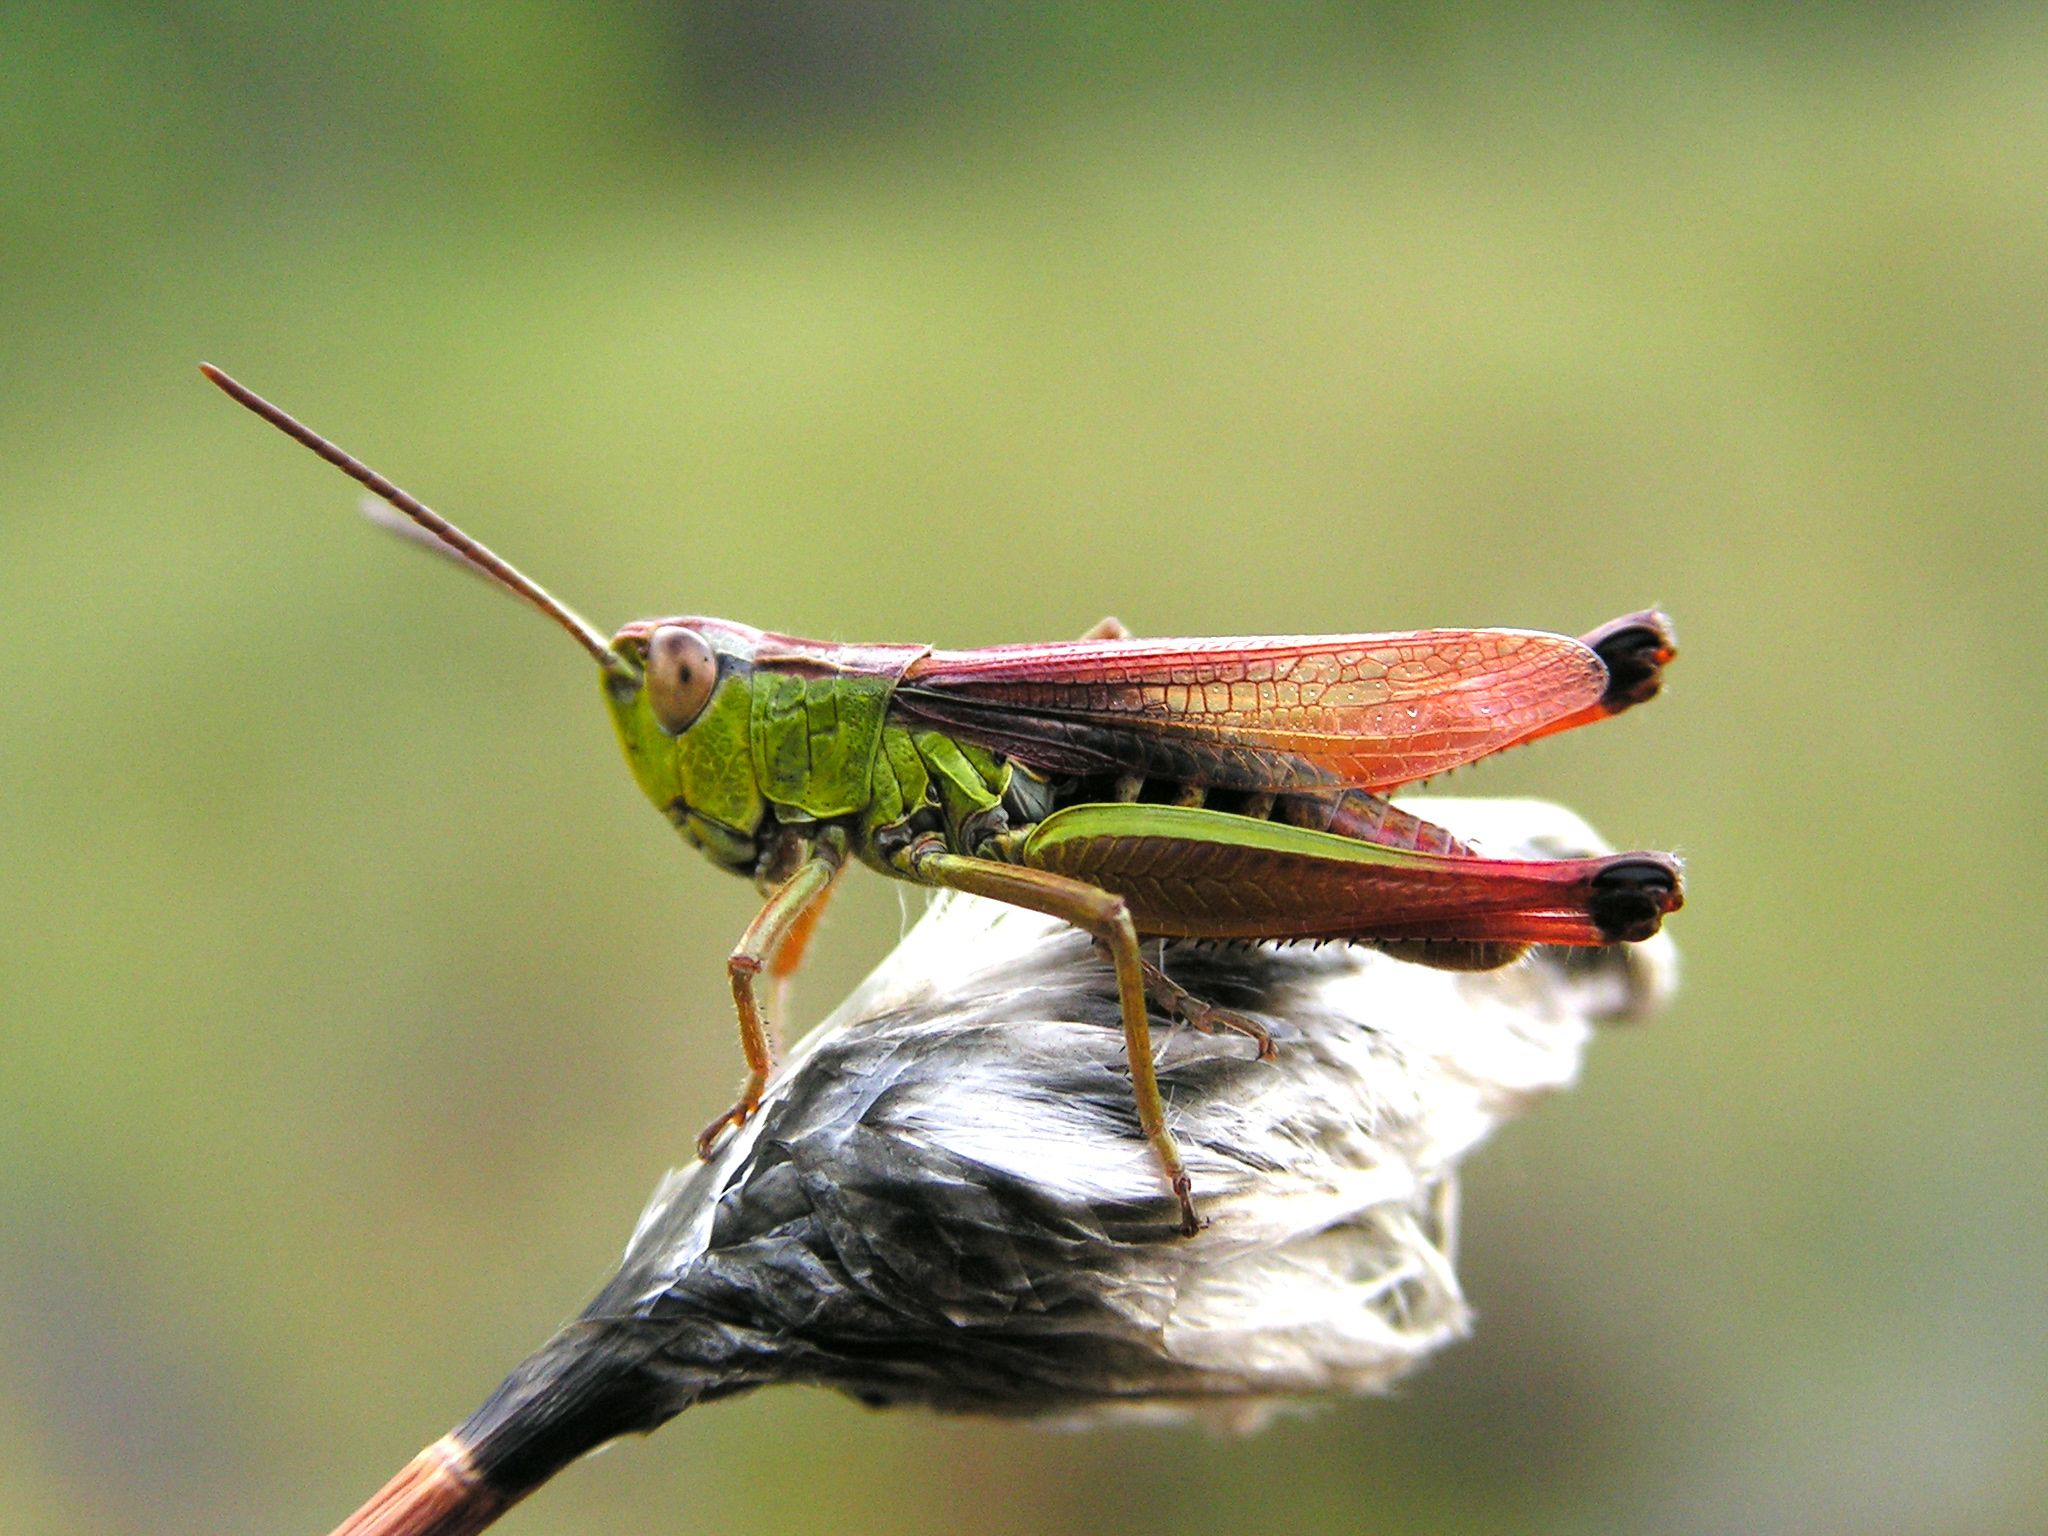
\includegraphics[width=\paperwidth]{grasshopper}}%
\frame{
\titlepage	% this creates the title page with the info provided before the beginning of the document
}
}
%%%%%%%%%%%%%%%%%%%%%%%%

\begin{frame}{Hybrid zone}
\begin{center}
\includegraphics[width=.9\textwidth]{map_of_hybrid_zone}
\end{center}
\end{frame}

%\begin{frame}{Background}
%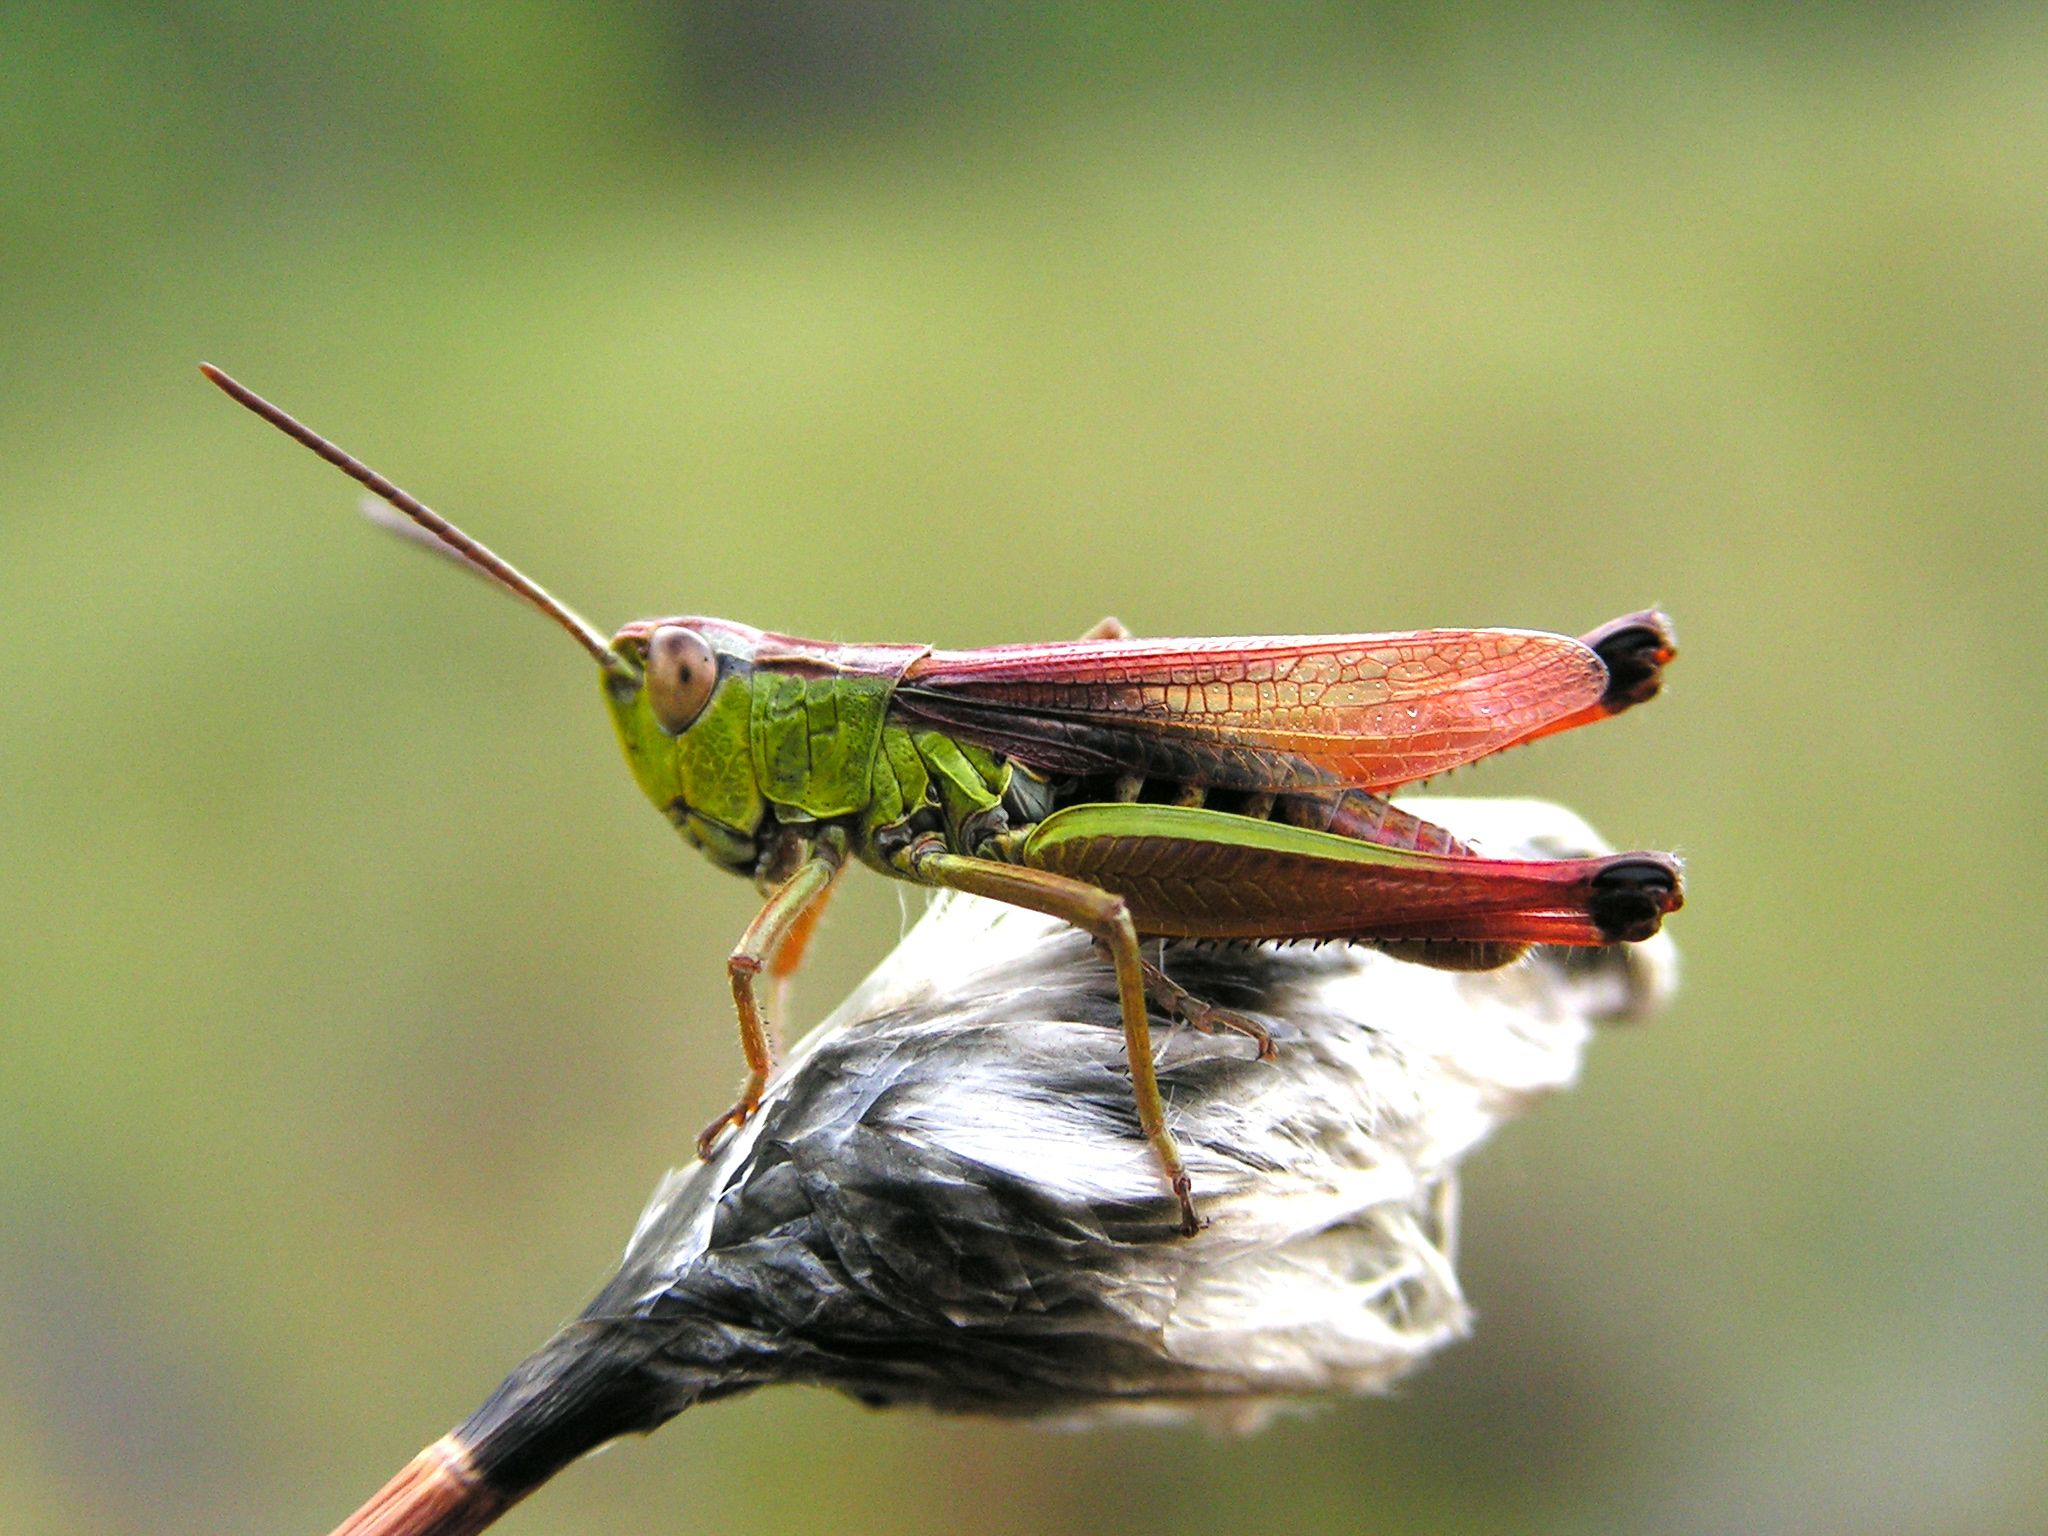
\includegraphics[width=\textwidth]{grasshopper}
%\end{frame}

\begin{frame}{each restriction site produces two tightly linked RAD tags}
\begin{center}
\begin{description}
\footnotesize
\item[RAD tag] marker locus; one of the sequences upstream or downstream of the restriction site
\end{description}
\vskip15pt
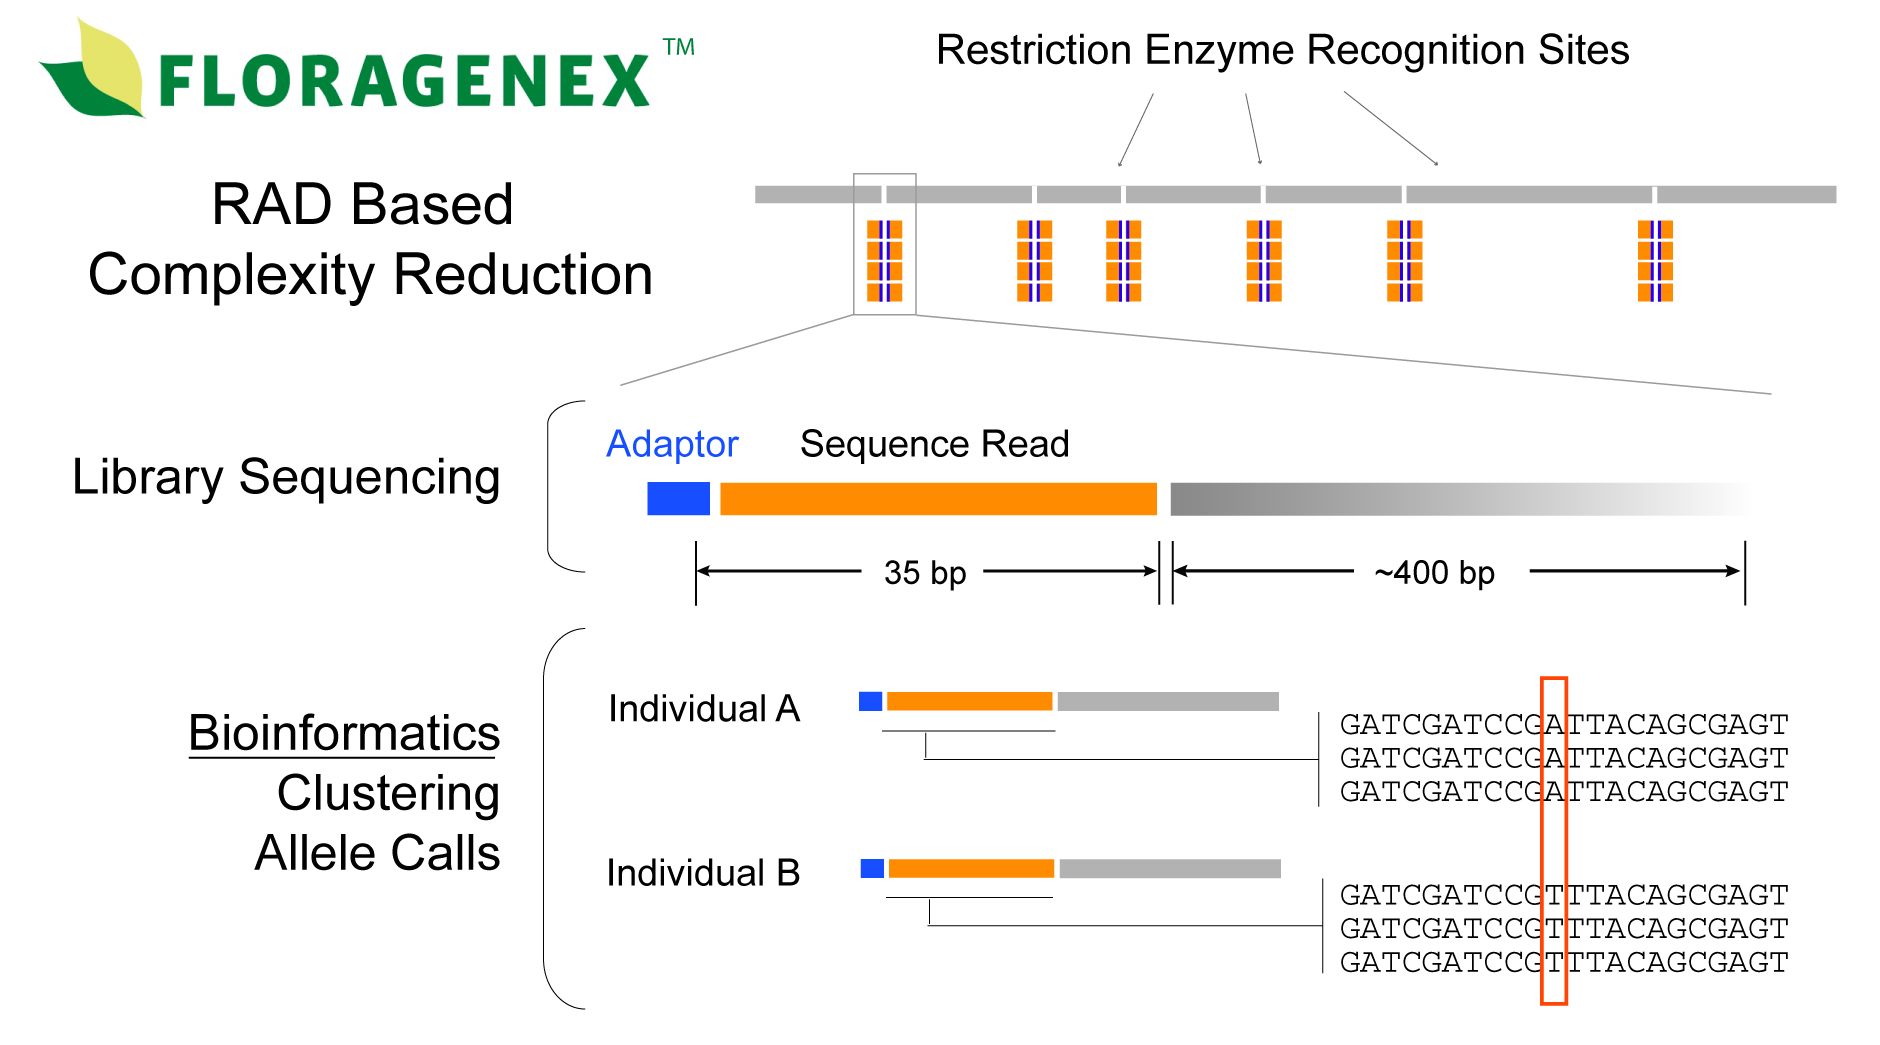
\includegraphics[height=.6\textheight]{RADprocessoverview}
\begin{block}{}
\centering
\scriptsize
reduced representation of the genome results in higher read coverage as compared to whole genome sequencing given the same amount of sequencing effort
\end{block}
\end{center}
\end{frame}
%
%
%
\begin{frame}[label=sRAD]{RAD \`a la \cite{Baird2008}}
\centering
\begin{columns}
\column{.6\textwidth}
\uncover<1->{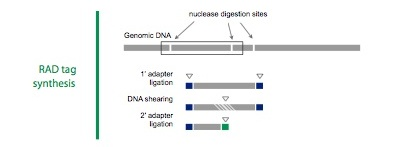
\includegraphics[width=\textwidth]{RADprotocolOverview_1}}
\uncover<2->{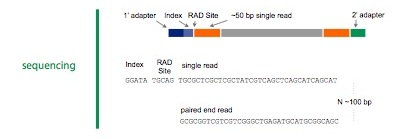
\includegraphics[width=\textwidth]{RADprotocolOverview_2}}
\uncover<3->{
\includegraphics[width=\textwidth]{RADprotocolOverview_3}}
\column{.5\textwidth}
\begin{itemize}[<+->]
\scriptsize
\item<1-> one restriction enzyme \smallskip
\item<1-> pooling of samples after ligation of first adapter \smallskip
\item<1-> random shearing of fragments before gel size selection \\
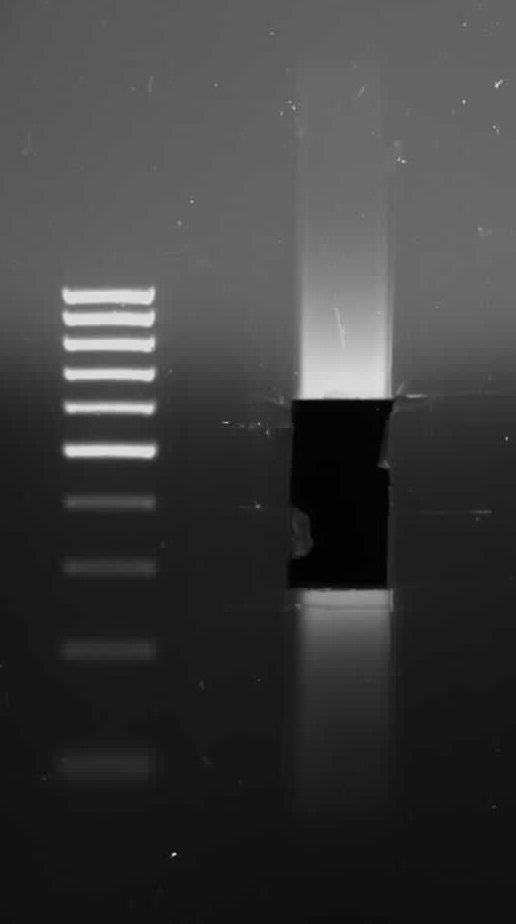
\includegraphics[width=.3\textwidth]{SizeSelection_180610} \smallskip
\item<2-> selective PCR after ligation of second adapter \smallskip
\item<2-> only fragments with at least one P1 adapter get amplified \smallskip
\item<3-> paired-end contig can be assembled for blasting
\end{itemize}
\end{columns}
\end{frame}

\begin{frame}{the fundamental problem}
\framesubtitle{dominance of singleton loci in the \texttt{stacks} assembly}
\vskip25pt
\begin{columns}
\column{.5\textwidth}
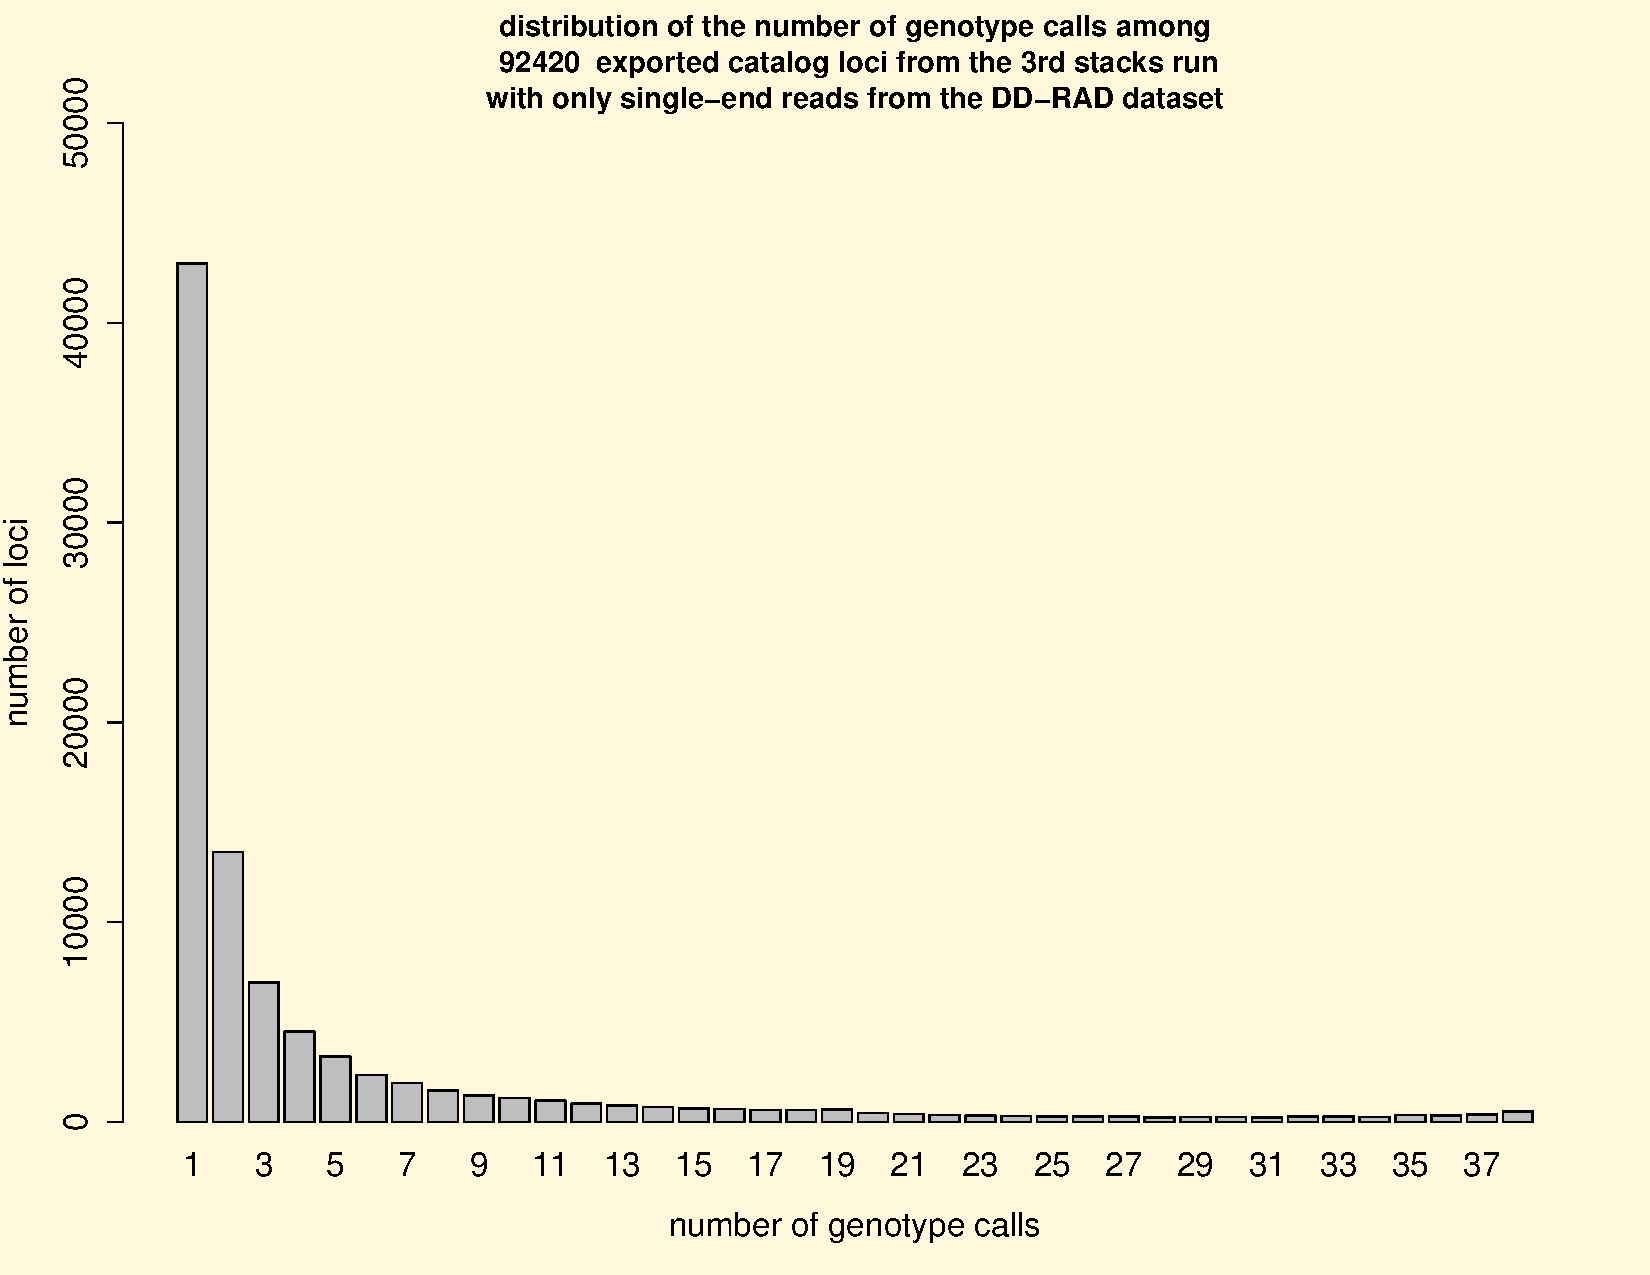
\includegraphics[width=\textwidth]{dist_geno_calls}
\column{.5\textwidth}
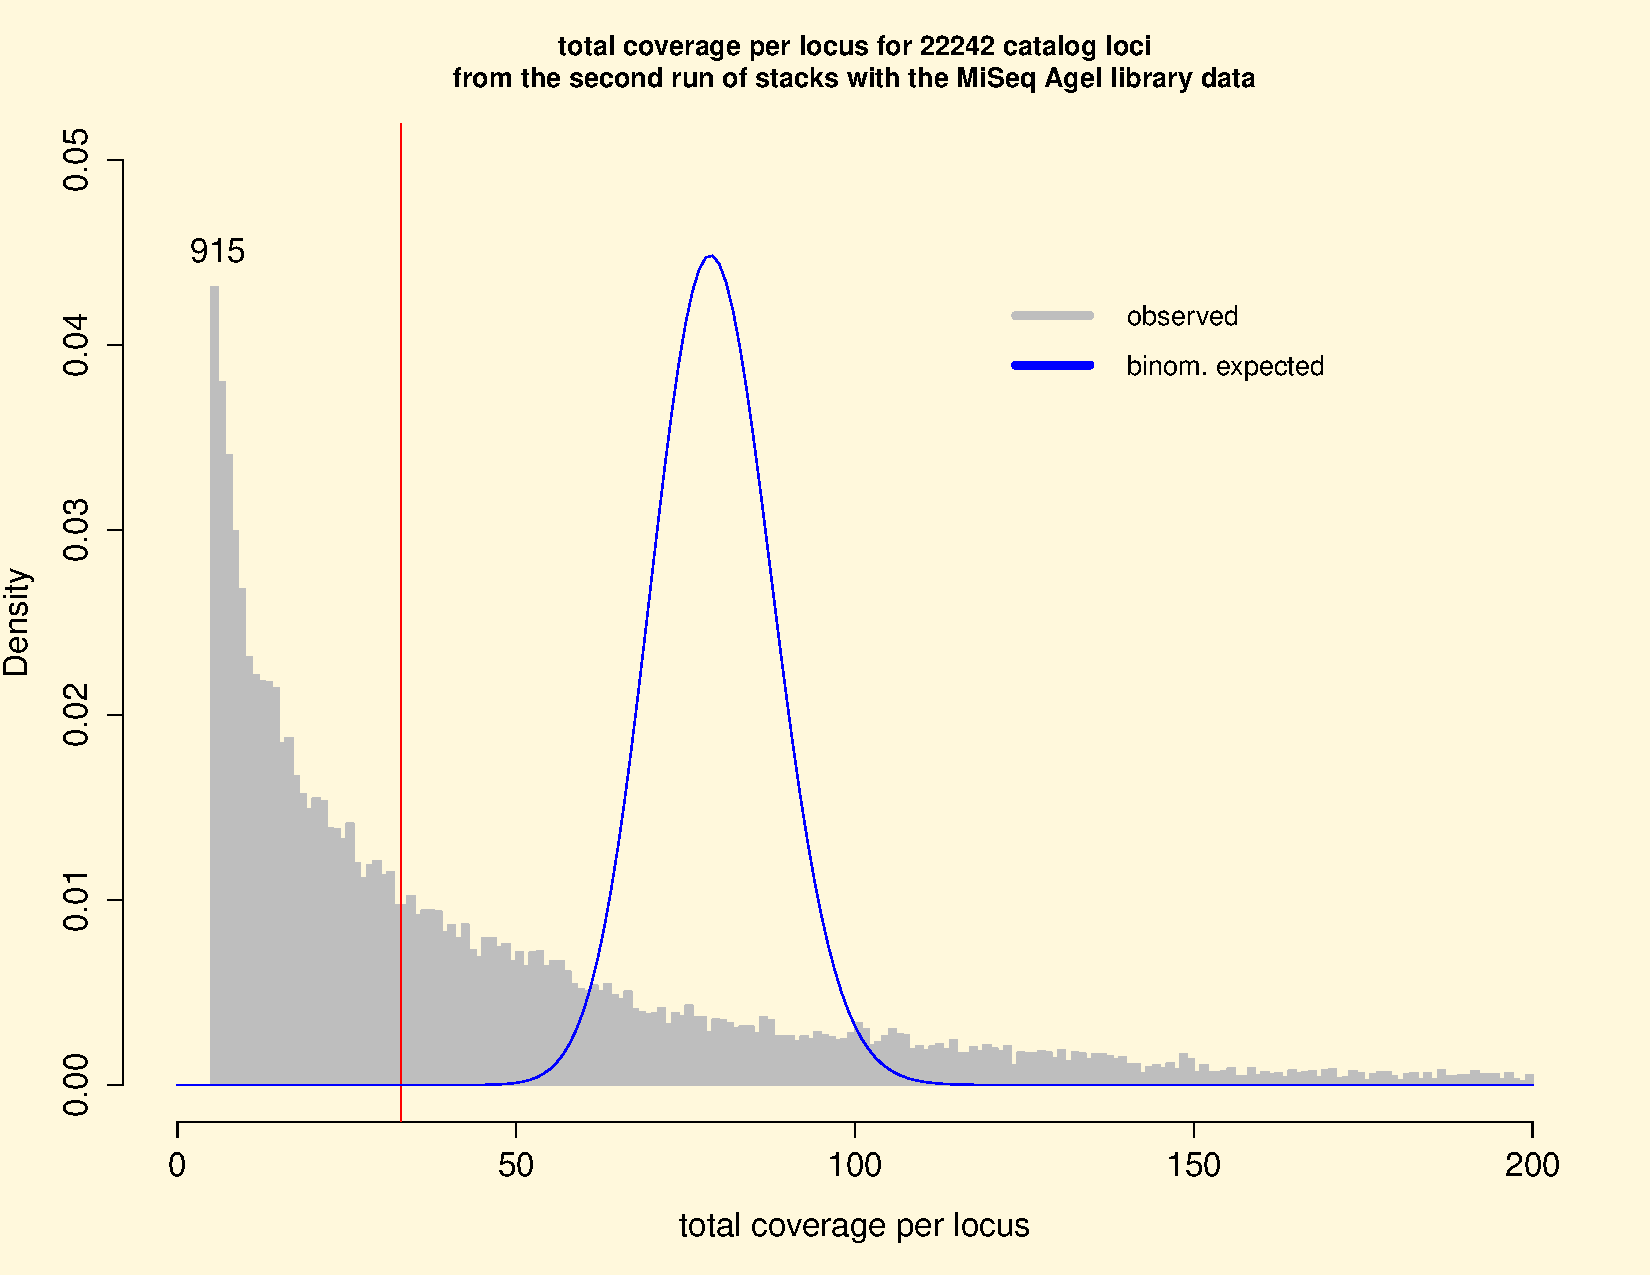
\includegraphics[width=\textwidth]{MiSeq_dist_of_cov}
\end{columns}
\vskip25pt
\begin{block}{}
\centering
What could be the reason for this result?
\end{block}
\end{frame}

\begin{frame}{a strange observation}
\centering
\footnotesize
0.034\% of quality filtered reads contain an SbfI recognition site
\vskip15pt
\begin{columns}
\column{.5\textwidth}
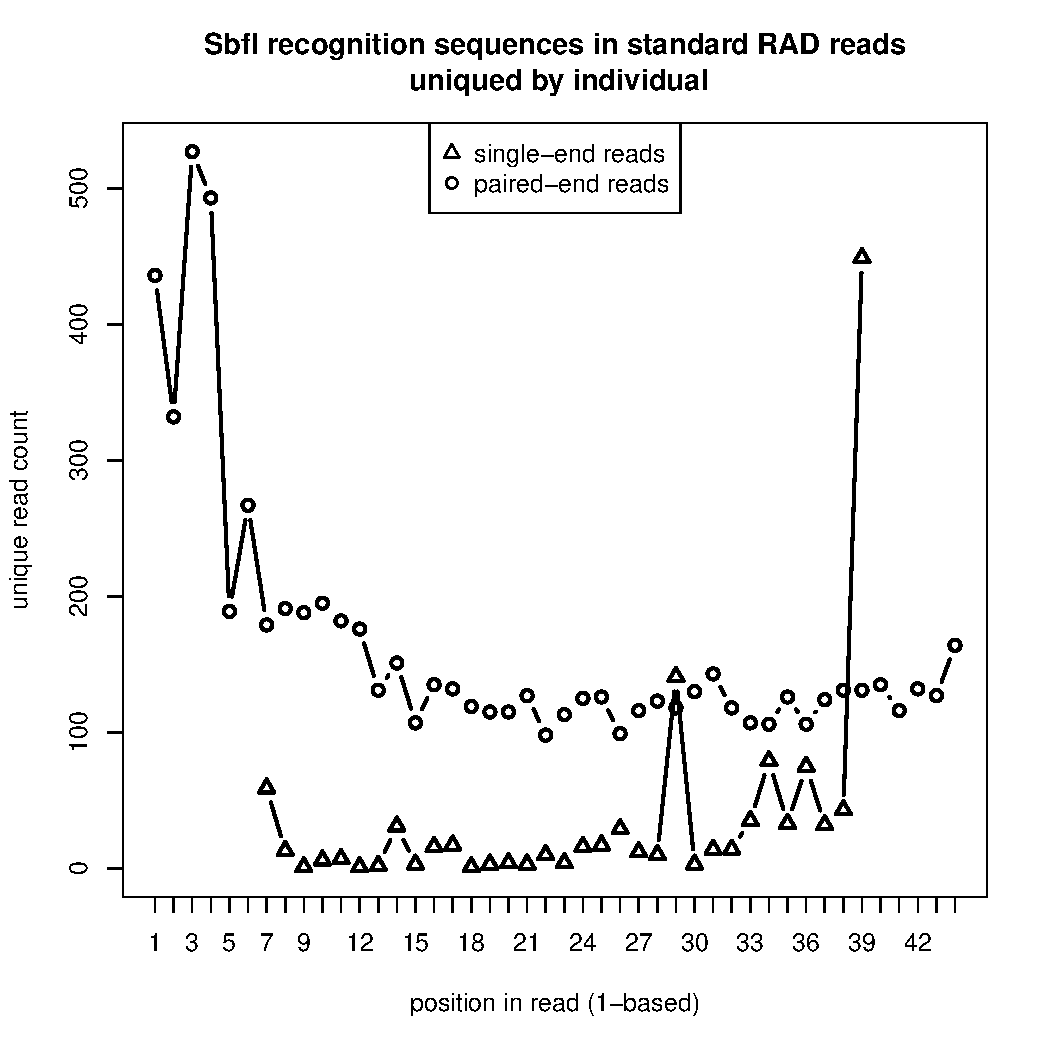
\includegraphics[width=\textwidth]{SbfI_positions_in_uniqued__by_ind___reads-1}
\column{.5\textwidth}
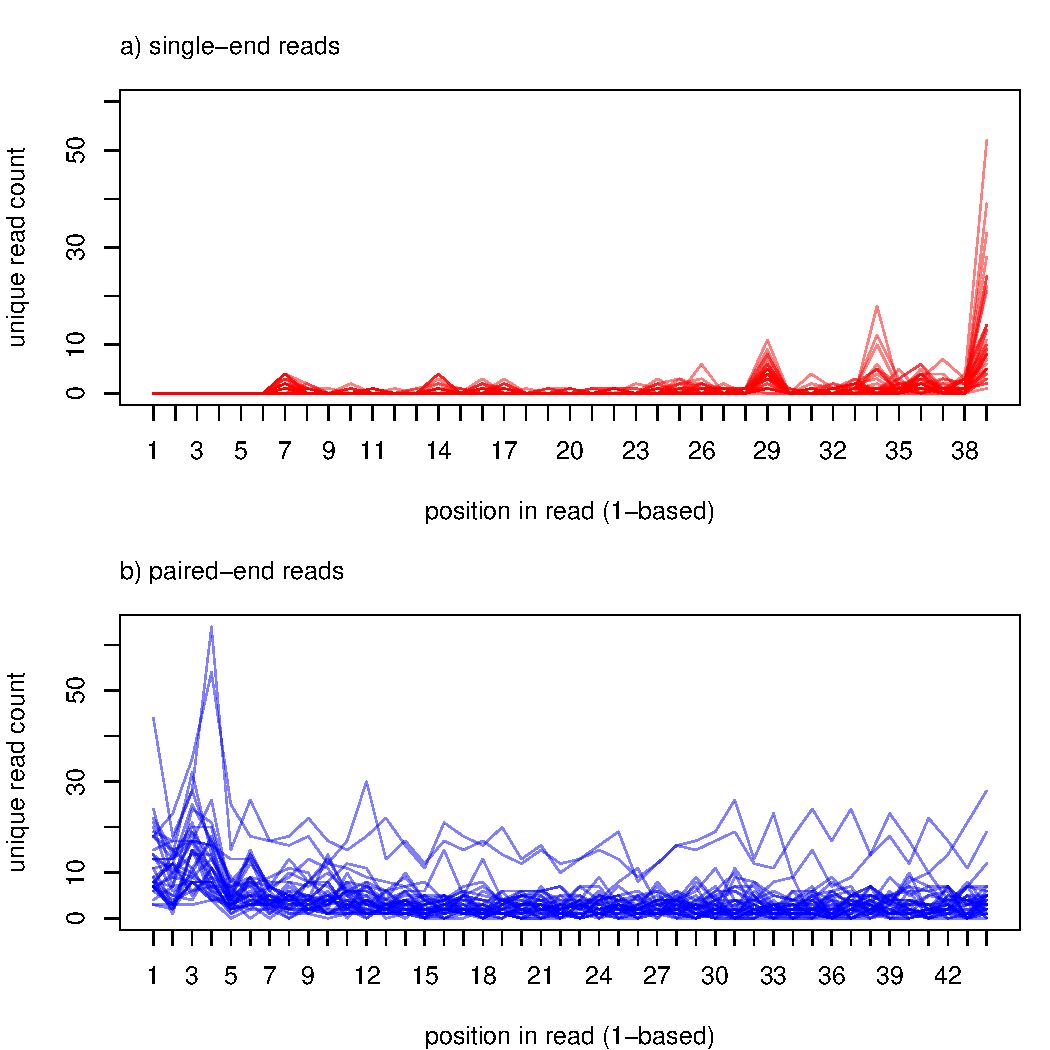
\includegraphics[width=1.1\textwidth]{SbfI_frequency_dist__per_ind_-1}
\end{columns}
\medskip
\pause
\begin{block}{}
\centering
Could this indicate incomplete digestion?
\pause
$\Rightarrow$ could be tested with PCR over restriction sites
but no reference sequence to design PCR primers
\end{block}
\end{frame}

\begin{frame}[shrink]
\frametitle{a locust transcriptome as reference}
\medskip
\scriptsize
from the migratory locust \textit{Schistocerca gregaria}
\medskip
\begin{center}
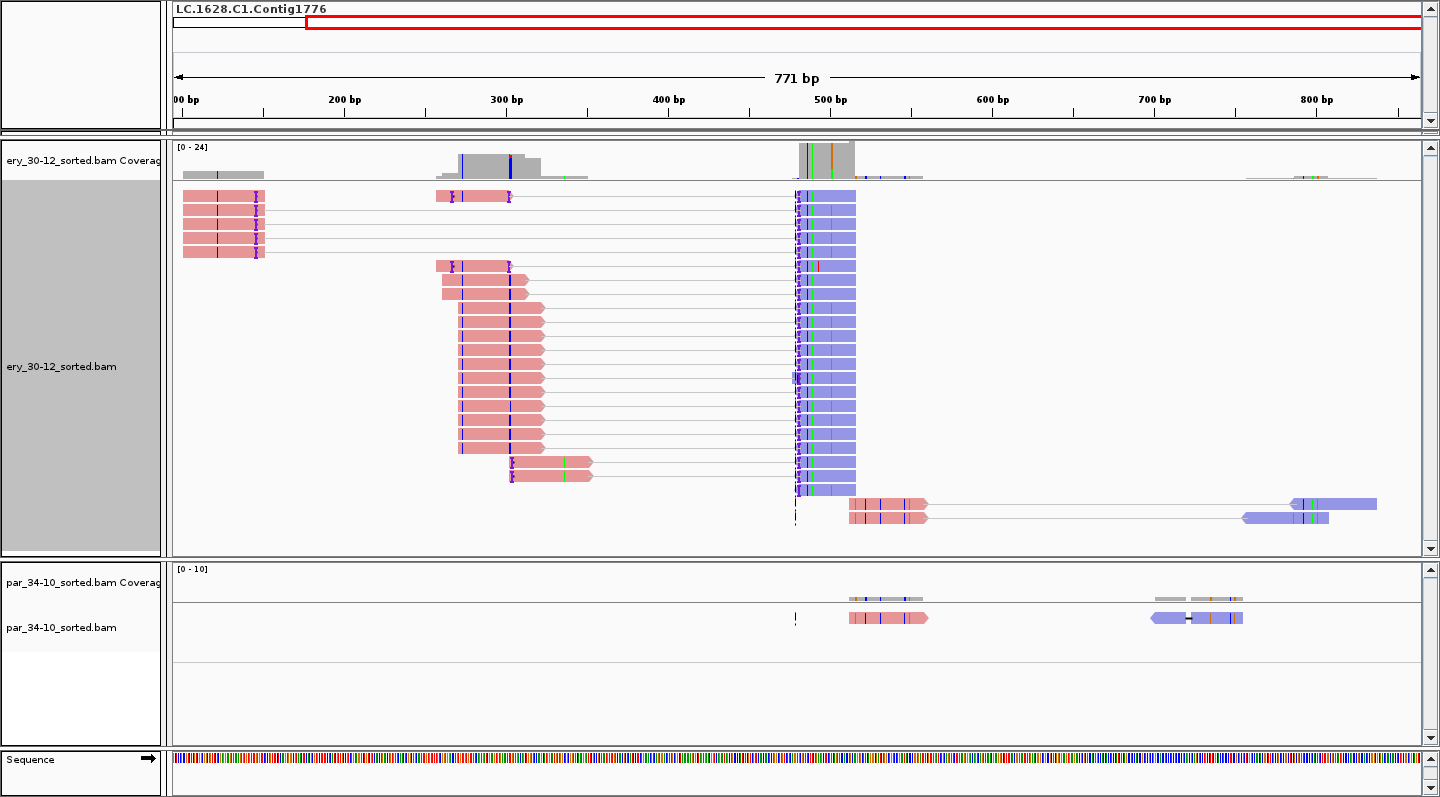
\includegraphics[width=.8\textwidth]{igv_LC_1628_C1_Contig1776_standRAD}
\end{center}
\pause
\begin{description}
\scriptsize
\item[linked RAD tag site] detected if there is at least one "properly mapped" read pair on either side of an SbfI restriction site
\end{description}
\pause
collect all paired-end reads whose single-end mate mapped to a detected \textrm{linked RAD tag} site
$\Rightarrow$ assembly into contigs
\end{frame}

\begin{frame}{}
\begin{itemize}
\item detected 77 \textit{Schistocerca} reference contigs with linked RAD tags site \pause \vskip10pt
\item chose assembler programme \texttt{SSAKE} because it can be set to allow low coverage for contig extension \pause \vskip10pt
\item \texttt{SSAKEoptimiser.pl} to find optimal kmer length for each individual assembly, optimisation for length of longest contig assembled \pause \vskip10pt
\item 64 \textit{Schistocerca} reference contigs with a RADtag site for which at least one upstream and one downstream \texttt{SSAKE} contig could be assembled
\end{itemize}
\end{frame}

\begin{frame}{parallelising the search for the optimal kmer length}
\begin{center}
\vskip -20pt
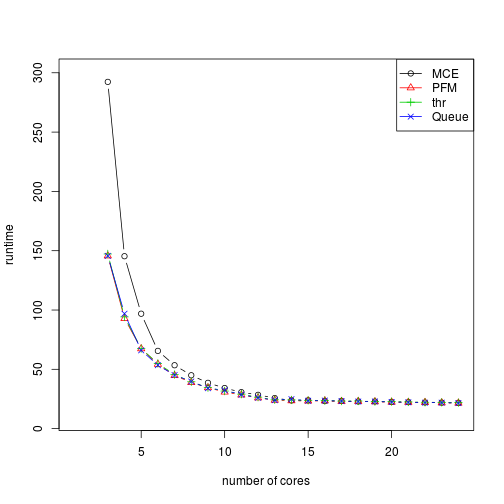
\includegraphics[width=.8\textwidth]{SSAKEoptimiser_runtimes}
\end{center}
\end{frame}

\begin{frame}{manual merging of \texttt{SSAKE} contigs}
variation in input sequences interferes with contig assembly\\ \vskip 15pt
\begin{center}
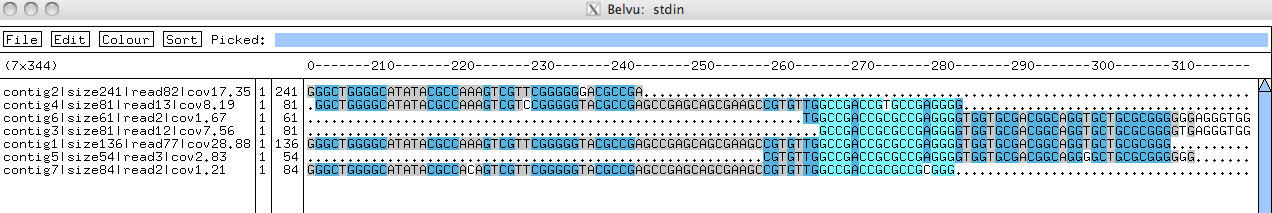
\includegraphics[width=\textwidth]{contig_alignment}
\end{center}
\end{frame}

\begin{frame}{picking the right \texttt{SSAKE} contig}
\footnotesize
\texttt{SSAKE} generally assembles many contigs for a given set of sequences\\ \vskip15pt
\texttt{blast} of \texttt{SSAKE} contigs against their putative \textit{Schistocerca} reference contig\\ \vskip15pt
\begin{center}
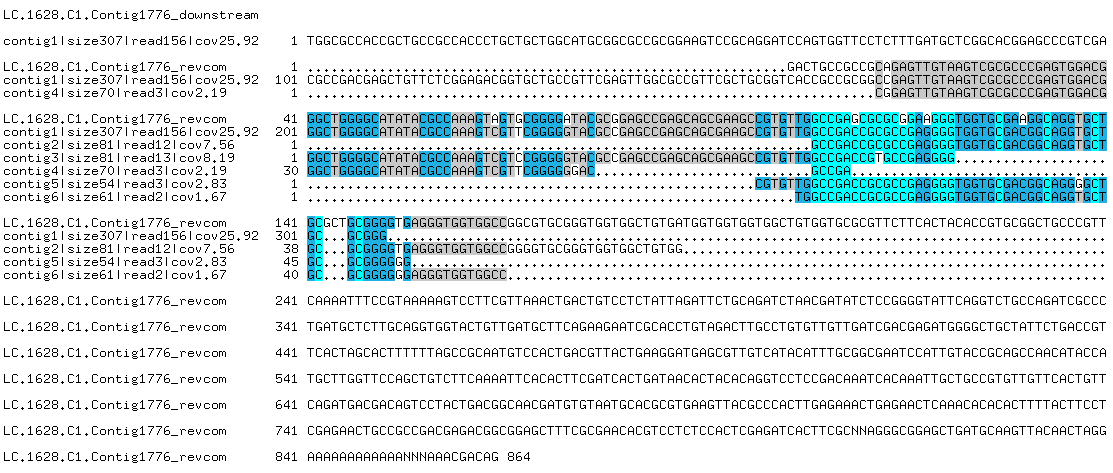
\includegraphics[width=.9\textwidth]{SSAKE_contigs_aligned_against_Schisto_contig}
\end{center}
check that the assembled upstream and downstream \texttt{SSAKE} contigs actually belong to the same locus, i. e. RADtag site
\end{frame}

\begin{frame}
\footnotesize
\begin{itemize}
\item for 20 \texttt{Schistocerca} cDNA contigs I could assemble and confidently pick down and upstream contigs for PCR primer design \pause
\item backmapping of reads against this new small reference made up of pairs of PE contigs $\Rightarrow$ \textrm{targeted alignment} \pause
\begin{center}
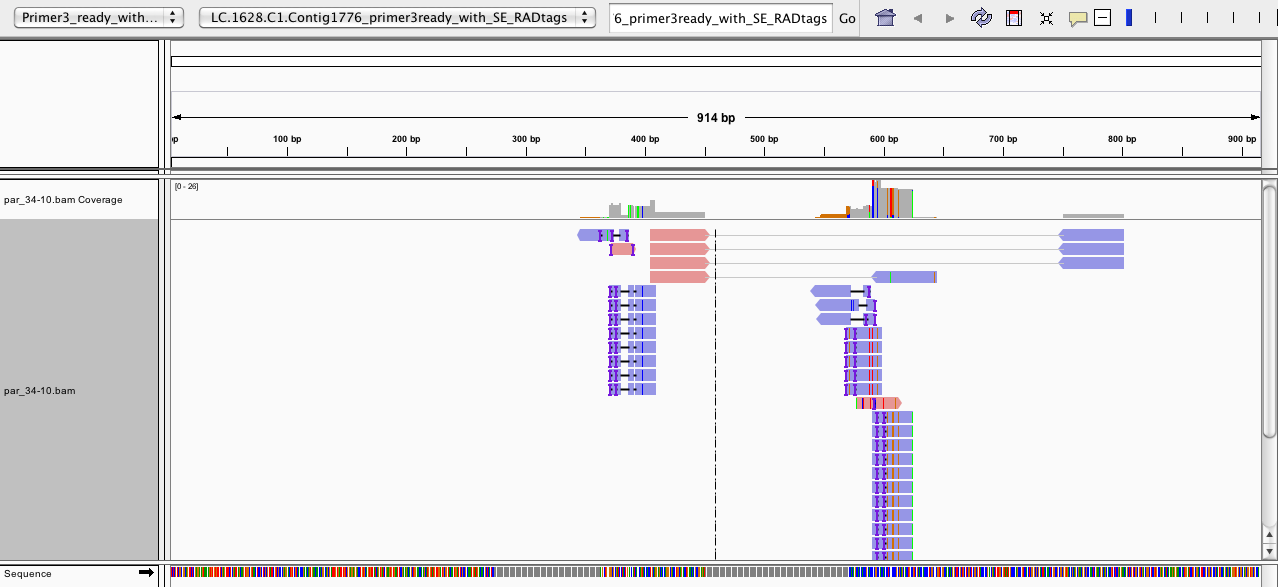
\includegraphics[width=\textwidth]{stampy_par_34-10_vs_primer3ready_igv}
\end{center} 
\pause
\item \texttt{Coval-refine}
\end{itemize}
\end{frame}

\begin{frame}{Coval-refine}
\begin{columns}
\column{.1\textwidth}
after
\vskip50pt
before
\column{.9\textwidth}
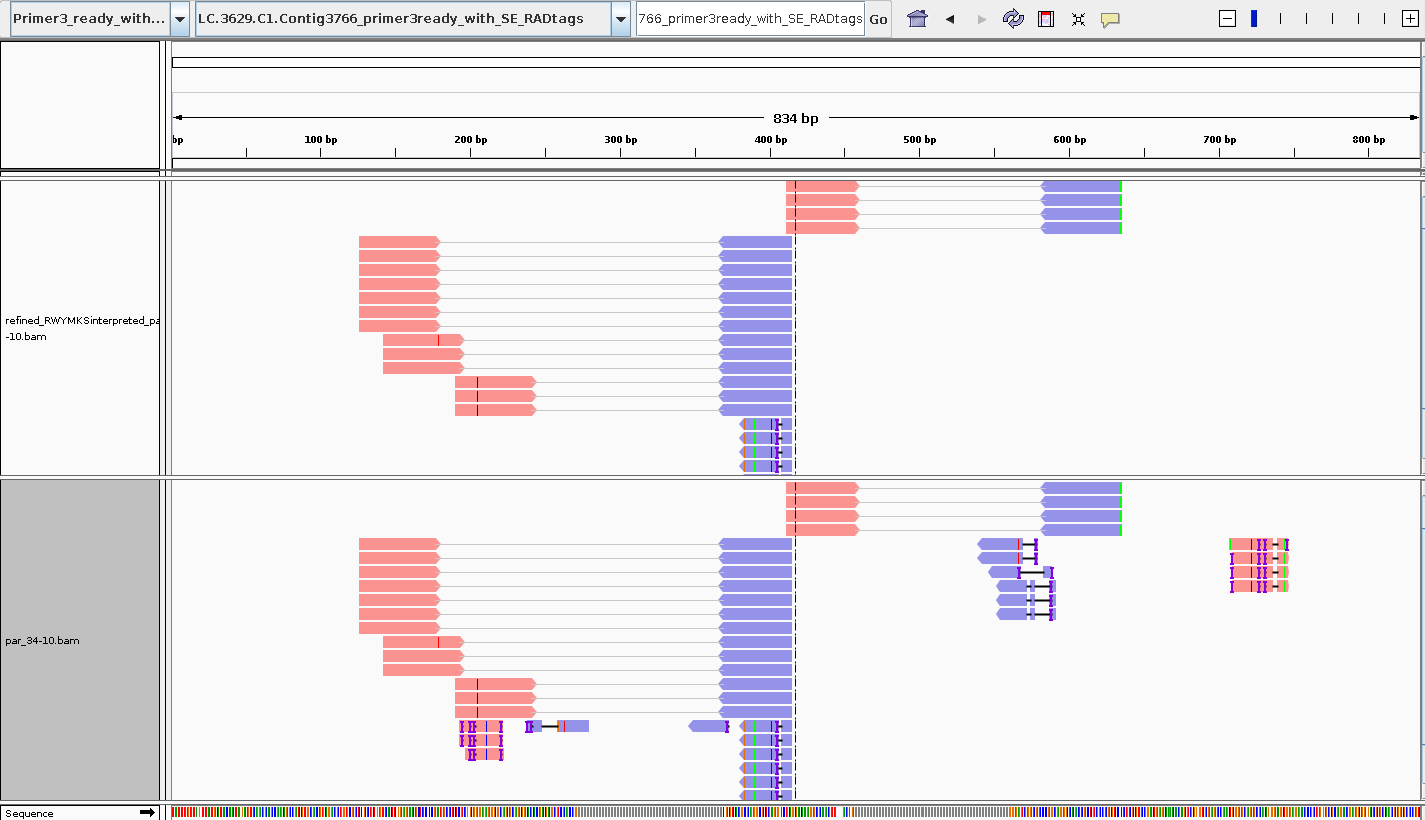
\includegraphics[width=\textwidth]{stampy_par_34-10_vs_primer3ready_after_coval-refine_igv}
\end{columns}
\end{frame}

\begin{frame}{Backmapping results}
\begin{columns}
\column{.6\textwidth}
\begin{center}
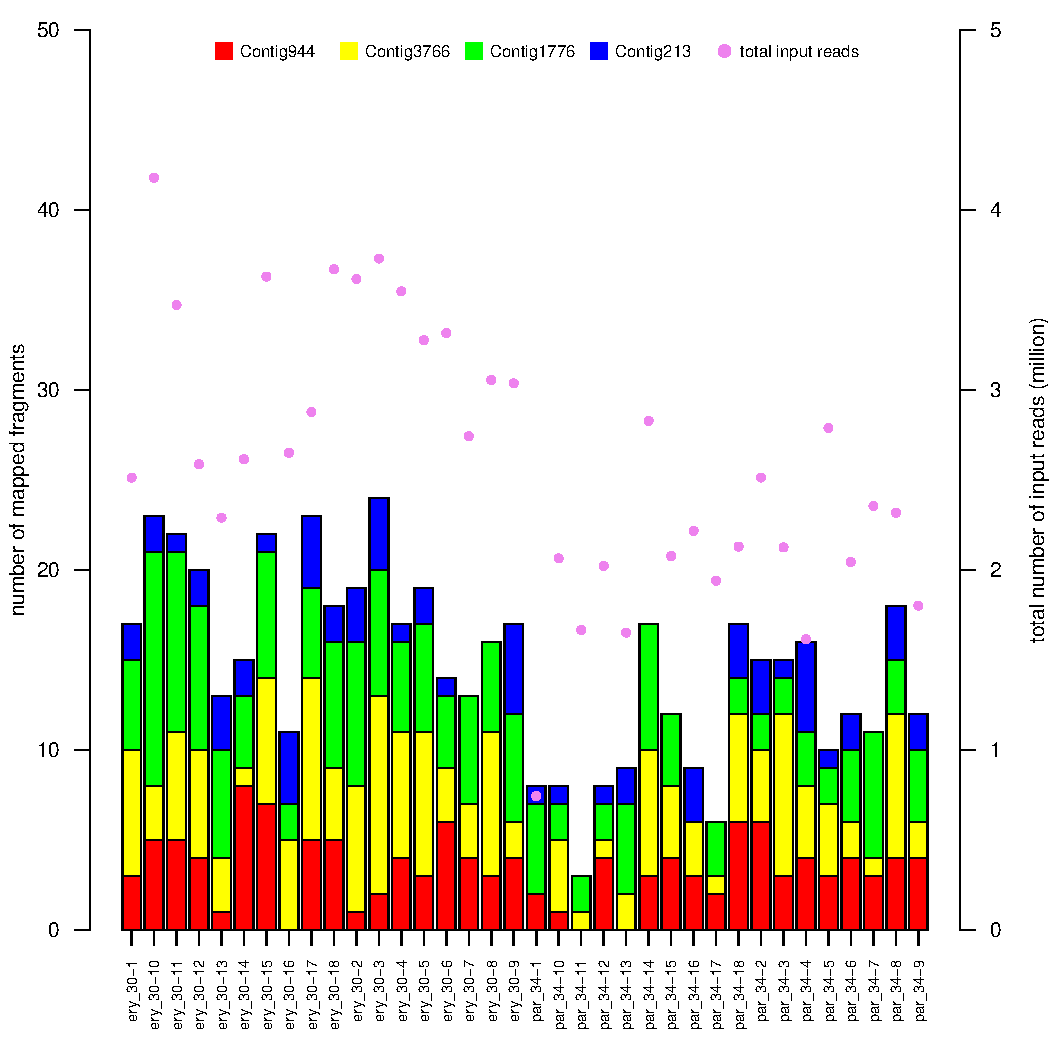
\includegraphics[width=\textwidth]{fragments_mapped_per_ind-1}
\end{center}
\pause
\column{.4\textwidth}
rather even fragment number from all individuals \\
$\Rightarrow$ incomplete digestion is unlikely to be the reason for the dominance of singleton loci in the \texttt{stacks} assembly
\end{columns}
\begin{description}
\vskip15pt
\centering
\scriptsize
\item [fragment] non-PCR duplicate
\end{description}
\end{frame}


\begin{frame}
\centering
\footnotesize
Does the number of reads mapped back from an individual to the PE contig reference correlate with the total read number of reads from that individual?
\vskip20pt
\begin{columns}
\column{.5\textwidth}
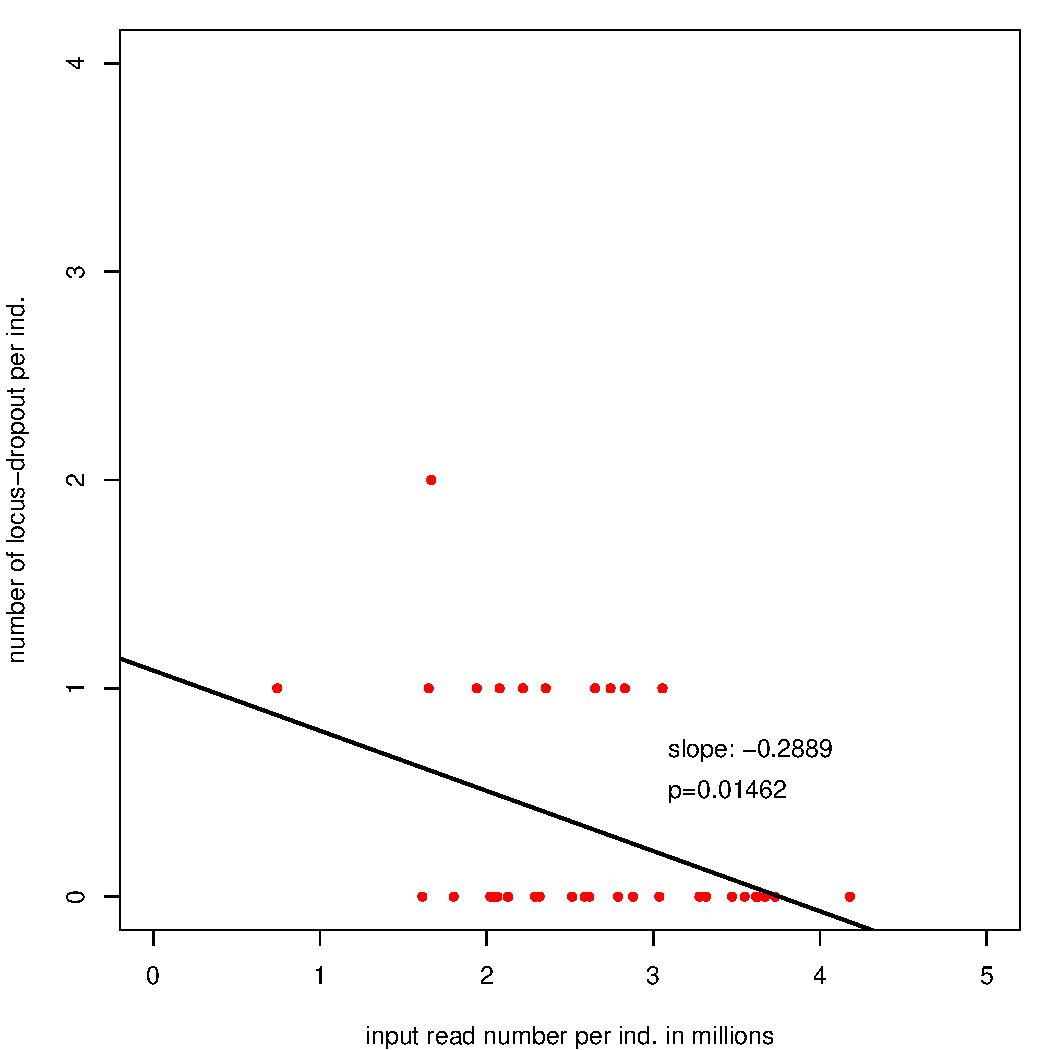
\includegraphics[width=\textwidth]{frag_input_corr_fig-1}
\column{.5\textwidth}
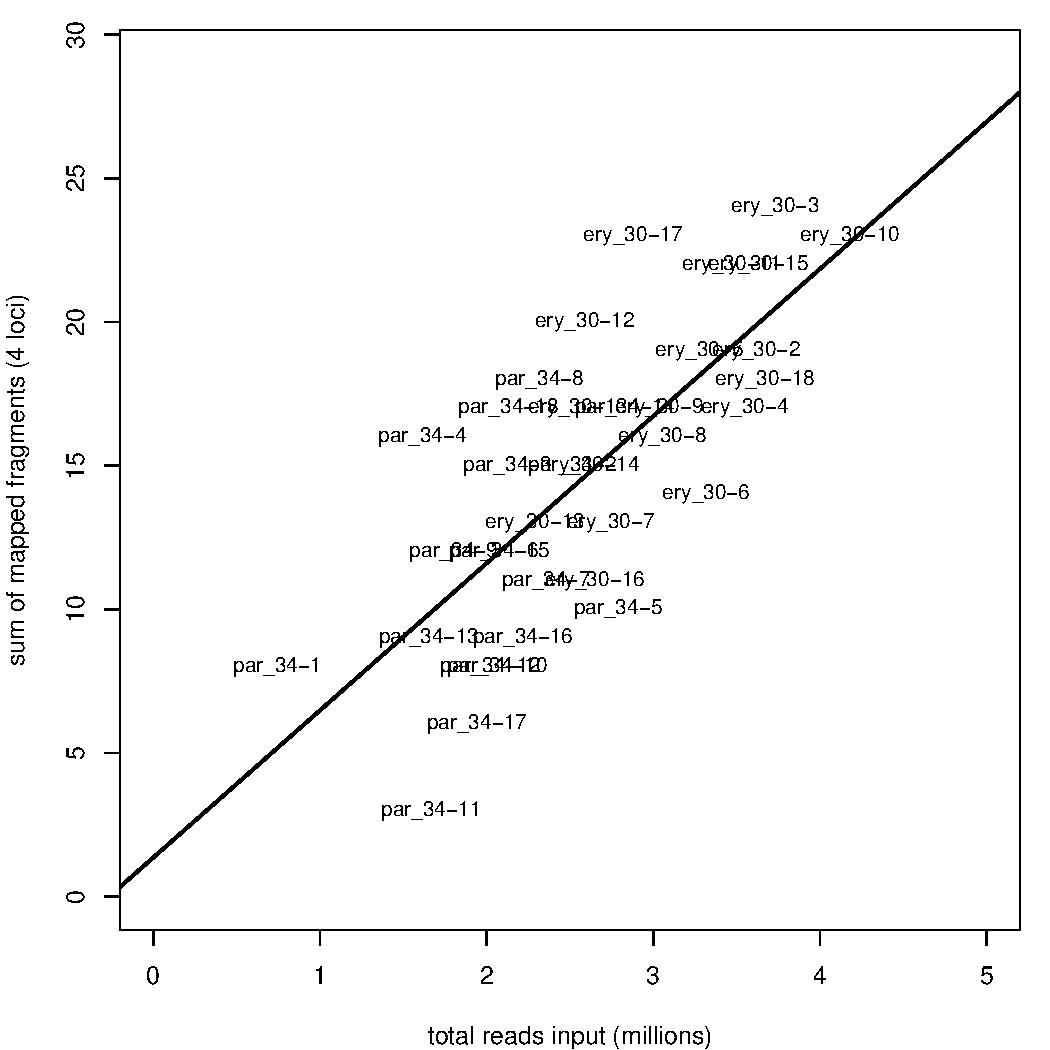
\includegraphics[width=\textwidth]{frag_input_corr_fig-2}
\end{columns}
\vskip20pt
\end{frame}

\begin{frame}
%\centering
\footnotesize
Could this problem be alleviated with sequencing more reads from the same library? 
\begin{center}
\includegraphics[width=0.7\textwidth]{PCR_duplicates}
\end{center}
\vskip10pt
Or, could low PCR template amount explain dominance of singleton loci in RAD tag assembly?
\end{frame}

\begin{frame}
\footnotesize
{\color{RoyalBlue!80}{If I added 100 ng of grasshopper DNA to the PCR mix, assuming that the genome is 12 Gbp long, this would only correspond to 7604 template molecules for the primers.}}
\vskip20pt
\begin{align}
\text{molar amount of template} &= \frac{\text{amount of DNA}}{\text{MW of bp} \times \text{genome size}} \nonumber \\[10pt]
&= \frac{100 \times 10^{-9}g}{660 \frac{g}{mol \times bp} \times 12 \times 10^{9} \text{bp}} \nonumber \\[10pt]
&= 1.26 \times 10^{-20} \text{mol} \nonumber
\end{align}
\begin{align}
\text{number of template molecules} &= 1.26 \times 10^{-20} \text{mol} \times \text{Avogadro's number} \nonumber \\[10pt]
&= 1.26 \times 10^{-20} \text{mol} \times 6.0221413 \times 10^{23} \nonumber \\
&= 7604 \nonumber
\end{align}
\end{frame}

\begin{frame}
\centering
SbfI sites in reads due to fragment-to-fragment re-ligation?
\end{frame}


%------------------------------------------------------------------------------------------

\begin{frame}[allowframebreaks] % the option "allowframebreaks" is very handy for spreading content over several slides
\frametitle{For Further Reading}
\scriptsize
\bibliographystyle{elsarticle-harv}
\bibliography{/Users/Claudius/Documents/MyLiterature/Literature}
\end{frame}


%------------------------------------------------------------------------------------------
% Example Slides and showcases
%------------------------------------------------------------------------------------------

%%%%%%%%%%%%%%%%%%%%%%%%%%%%%
%% overlays
%%%%%%%%%%%%%%%%%%%%%%%%%%%%%
%\frame
%{
%  \frametitle{Features of the Beamer Class}
%%  \framesubtitle{}
%  \begin{itemize}
%  \item<1-> Normal LaTeX class.
%  \item<2-> Easy overlays.
%  \item<3-> No external programs needed.      
%  \end{itemize}
%}
%%%%%%%%%%%%%%%%%%%%%%%%%%%%%

%%%%%%%%%%%%%%%%%%%%%%%%%%%%%
%% examples of `block` types
%%%%%%%%%%%%%%%%%
%\begin{frame}{Block types}
% 
%   \begin{block}{This is a Block}
%      This is important information
%   \end{block}
%
% 	\vskip20pt
%
%   \begin{alertblock}{This is an Alert block}
%   This is an important alert
%   \end{alertblock}
% 
%   \begin{exampleblock}{This is an Example block}
%   This is an example 
%   \end{exampleblock}
% 
%\end{frame}
%%%%%%%%%%%%%%%%%%%%%%%%%%%%%

%%%%%%%%%%%%%%%%%%%%%%%%%%%%%
% dividing the slide into columns
%%%%%%%%%%%%%%%%%%%%%%%%%%%%%%
%\begin{frame} 
%\frametitle{Two Column Output}
%\begin{columns}[c] 
%\column{.5\textwidth} 
%Practical \TeX\ 2005\\
% \vskip20pt
%Practical \TeX\ 2005\\ 
%Practical \TeX\ 2005
%\column{.5\textwidth} 
%\includegraphics[width=\textwidth]{/Users/Claudius/Documents/PhD/Presentations/journal_club/Orozco2012/PNG/isofemale_line.pdf}
%\end{columns}
%\end{frame}
%%%%%%%%%%%%%%%%%%%%%%%%%%%%%

%%%%%%%%%%%%%%%%%%%%%%%%%%%%%
% Definitions:
%%%%%%%%%%%%%%%%%%%%%%%%%%%%%%
%\frame{
%\frametitle{how to give a definition of a word}
%\begin{description}
%\item[isofemale line] a line started from a single mated female
%\end{description}
%}
%%%%%%%%%%%%%%%%%%%%%%%%%%%%%

%%%%%%%%%%%%%%%%%%%%%%%%%%%%%
% % table with row colors
%%%%%%%%%%%%%%%%
%\begin{frame}[fragile]
%testcolors
%\frametitle{A table with alternating row colors}
%\small
%In order for this to work, call the \textrm{beamer} class with the following options:
%\begin{verbatim}
%\documentclass[xcolor=pdftex, dvipsnames, table]{beamer}
%\end{verbatim}
%\vskip20pt
%\begin{center}
%\rowcolors{1}{RoyalBlue!20}{RoyalBlue!5} % these are `dvipsnames` from the xcolor package
%\begin{tabular}{lccr}
%\toprule
%This & is & the & header \\ [5pt]
%\midrule
%This & is the & content of & the first line \\
%This & is the & content of & the second line \\
%\bottomrule
%\end{tabular}
%\end{center}
%\vskip20pt
%The \colorbox{yellow}{rowcolors} command has to come right before the \textrm{tabular} environment.
%% The `rowcolors` command is provided by the `xcolor` package.
%\end{frame}
%%%%%%%%%%%%%%%%%%%%%%%%%%%%%

%%%%%%%%%%%%%%%%%%%%%%%%%%%%%
% overlays with \pause
%%%%%%%%%%%%%%%%%
%\begin{frame}[fragile] % the fragile option to the frame command is necessary if you want to use `verbatim` environments.
%\frametitle{Overlays with {\tt pause}}
%
%\setbeamercovered{dynamic}
%% overlays not yet revealed will faintly appear. Use "invisible" to turn that off.
%The command:
%\begin{verbatim}
%\setbeamercovered{dynamic} 
%\end{verbatim}
%\ldots allows overlays not yet revealed to be already faintly appear.
%\vskip20pt
%Practical \TeX\ 2005\\ \pause 
%Practical \TeX\ 2005\\ \pause 
%Practical \TeX\ 2005 
%\\ this does also work for graphics? \\ 
%\end{frame}
%%%%%%%%%%%%%%%%%%%%%%%%%%%%%

%%%%%%%%%%%%%%%%%%%%%%%%%%%%%
%%
%%%%%%%%%%%%%%%%%%%%%%%%%%%%%
%\begin{frame}[fragile] 
%\frametitle{Tic-Tac-Toe via {\tt tabular} and \textrm{onslide}}
%Overlays that are not yet revealed can be made invisible by this command:
%\begin{verbatim}
%\setbeamercovered{invisible} 
%\end{verbatim}
%\vskip20pt
%{\Huge 
%\begin{center}
%\begin{tabular}{c|c|c} 
%\onslide<9->{O} & \onslide<8->{X} & \onslide<2->{X} \\ 
%\hline \onslide<6->{X} & \onslide<3->{O} & \onslide<5->{O} \\ 
%\hline \onslide<10->{X} & \onslide<7->{O} & \onslide<4->{X}
%\end{tabular} 
%\end{center} 
%} 
%\end{frame}
%%%%%%%%%%%%%%%%%%%%%%%%%%%%%

%%%%%%%%%%%%%%%%%%%%%%%%%%%%%%%
% a slide with references
%%%%%%%%%%%%
%Citations used on the previous slides should appear here.
%\begin{frame}[allowframebreaks] % the option "allowframebreaks" is very handy for spreading content over several slides
%\frametitle{For Further Reading}
%\scriptsize
%\bibliographystyle{elsarticle-harv}
%\bibliography{/Users/Claudius/Documents/MyLiterature/Literature}
%\end{frame}
%%%%%%%%%%%%%%%%%%%%%%%%%%%%%%%



%%		%%
%		
%
%
%
%
%%		%%


%%%%%%%%%%%%%%%%%%%%%%%%%%%
%% simple list with overlays and hyperlink
%%%%%%%%%%%%%%%%%%%%%%%%%%%
%\frame{
%\frametitle{Santa Rosalia}
%\begin{itemize}
%\item Why are there so many species on earth? \pause
%\vskip10pt
%\item Why aren't there even more? \pause
%\vskip10pt
%\item Ecological constraints to diversity? 
%	\begin{itemize}
%	\item competition between species ?
%	\item Can we expect lots of ecologically identical species ? 
%	\\ $\rightarrow$ \href{http://www.nature.com/scitable/knowledge/library/neutral-theory-of-species-diversity-13259703}{\color{RoyalBlue!80}{neutral theory of species diversity}} \pause
%	\end{itemize}
%\vskip10pt
%\item Evolutionary constraints to diversity? 
%	\begin{itemize}
%	\item additive genetic variation ?
%	\item gene flow ?
%	\item recombination ?
%	\item lack of recombination ?
%	\end{itemize}
%\end{itemize}
%}
%%%%%%%%%%%%%%%%%%%%%%%%%%%



%%%%%%%%%%%%%%%%%%%%%%%%%%%%%%%%%%%%%%%%%%%%
% frame subtitle
% quotation
% item list with custom item symbols
% subdivision with columns
% including a figure
% font size
% inserting custom space
%%%%%%%%%%%%%%%%%%%%%%%%%%%%%%%%%%%%%%%%%%%%
% in order to use pictures from papers: grab them with the `Grab` app and use the `ConvertToPNG` AppleScript to convert them to .png format. 
% The output of the script is in a folder called `PNG` on the desktop.
%\begin{frame}%[allowframebreaks]
%\frametitle{The haploid model}
%\framesubtitle{local adaptation --  postzygotic isolation}
%
%\footnotesize
%
%\vskip5pt
%
%\begin{quote}
%\ldots it is the simplest model I can find which exhibits many of the genetic effects which will be found in more complex, more realistic models of speciation.
%\end{quote}
%\begin{itemize}
%\item infinite$^{1}$ haploid$^{2}$ population with discrete$^{3}$ generations, i. e.
%	\begin{itemize}
%	\item [1] no genetic drift
%	\item [2] no heterozygous effects
%	\item [3] non-overlapping generations
%	\end{itemize}
%\item two loci for local adaptation --  B/b and C/c
%\end{itemize}
%
%\pause
%\vskip10pt
%
%\begin{columns}
%\column{.5\textwidth}
%%\includegraphics[width=\textwidth]{fig_1}
%\column{.5\textwidth}
%\begin{itemize}
%\item multiplicative combination of fitness effects across loci
%\item average fitness across habitats of genotypes \textit{BC} and \textit{bc} always greater than their recombinants
%\end{itemize}
%\end{columns}
%
%\end{frame}
%%%%%%%%%%%%%%%%%%%%%%%%%%%%%%%%%%%%%%%%%%%%%%%%%%%%



%%%%%%%%%%%%%%%%%%%%%%%%%%%%%%
% using the `shrink` option to the frame command 
% to allow more content to fit on the slide
%%%%%%%%%%%%%%%%%%%%%%%%%%%%%%
%\begin{frame}[shrink]
%\frametitle{The haploid model}
%\framesubtitle{assortative mating -- prezygotic isolation}
%
%\begin{itemize}
%\item assortative mating locus A/a
%\item $d$ is the proportion of individuals which mate positive assortatively, i. e. strength of assortative mating
%\end{itemize}
%
%\begin{center}
%%\includegraphics[width=.6\textwidth]{fig_2}
%\end{center}
%
%\begin{quote}
%The A locus controls the division of the mating pool into two mating groups according to space, time or phenotype. 
%\end{quote}
%
%\color{red}{Find biological examples for assortative mating according to \emph{space}, \emph{time} or \emph{phenoptype} directed by alleles at a \underline{single} locus!}
%
%\end{frame}
%%%%%%%%%%%%%%%%%%%%%%%%%%%%%%



%%%%%%%%%%%%%%%%%%%%%%%%%%%%%%
% dividing slide into columns
% table with `multicolumn` and `rowcolors`
%%%%%%%%%%%%%%%%%%%%%%%%%%%%%%
%\begin{frame}[shrink]
%\frametitle{Type of interaction between loci}
%\framesubtitle{multiplicative vs. additive combination of fitness effects}
%
%\scriptsize
%
%\vskip10pt
%
%\begin{columns}[t]
%
%\column{.5\textwidth}
%{\color{Green}multiplicative interaction}: \\[10pt]
%%\includegraphics[width=1.1\textwidth]{fig_1}
%\vskip10pt
%lower mean fitness of recombinant genotypes
%
%\column{.5\textwidth}
%{\color{Green}additive interaction}: \\[10pt]
%\begin{center}
%\rowcolors{3}{RoyalBlue!20}{RoyalBlue!5}
%\begin{tabular}{lcc}
%\toprule
% & \multicolumn{2}{c}{Habitat}  \\
%Genotype & I & II  \\ 
%\midrule
%BC & $1+2s$ & 1 \\
%Bc & $1+s$ & $1+s$ \\
%bC & $1+s$ & $1+s$ \\
%bc & 1 & $1+2s$ \\
%\bottomrule
%\end{tabular}
%\end{center}
%equal mean fitness of all genotypes
%
%\end{columns}
%
%\vskip10pt
%
%\begin{itemize}
%\item When $m=0.5$, i. e. in full sympatry, and with additive fitness combination, i. e. $\sim$ equal mean fitness of genotypes across habitats, no association between A and B-C can be established. \pause
%\item With reduced migration rates, i. e. parapatry, an association between A and B-C can be established with $\sim$ equal mean fitnesses of genotypes.
%\end{itemize}
%\pause
%\color{red}{Explain what multiplicative and additive interactions between loci mean in biological terms!}
%\end{frame}
%%%%%%%%%%%%%%%%%%%%%%%%%%%%%%



%%%%%%%%%%%%%%%%%%%%%%%%%%%%%%
% inserting a citation
%%%%%%%%%%%%%%%%%%%%%%%%%%%%%%
%\frame{
%\frametitle{Diskussion}
%\begin{itemize}
%\item Is the range of selection coefficients in the models realistic? $\rightarrow$ see \cite{Kingsolver2001}
%\item A lot of initial assortative mating is required in all models even with migration rates as low as 0.01. Is such a high level of assortative mating biologically plausible to exist in many species?
%\item What's the difference between the "one-allele" and "two-allele" model?
%\item How can one test for the occurrence of the "one-allele" model?
%\end{itemize}
%}
%%%%%%%%%%%%%%%%%%%%%%%%%%%%%%



%%%%%%%%%%%%%%
\end{document}
%%%%%%%%%%%%%